\documentclass[../Main.tex]{subfiles}

\begin{document}
\chapter{Machine \& Deep Learning}

\section{MLOps: Continuous Delivery and Automation pipelines in ML}

\textbf{Google DevOps} $\Rightarrow$ Applying DevOps philosophy to software development and infrastructure on the Google Cloud Platform (GCP)

\begin{itemize}
    \item \textbf{CI/CD:} Implementing automated pipelines with tools like Cloud Build and Container Registry to continuously integrate code changes and deliver software to production
    \item \textbf{Kubernetes (GKE):} Leveraging's Google's container orchestration platform, Kubernetes (and its managed service, GKE), to manage and deploy containerized application effectively
    \item \textbf{Observability:} Implementing practices and tool like \textit{Cloud logging} and \textit{Stackdriver} for monitoring, logging, and troubleshooting application and infrastructure in real-time
    \item \textbf{Site Reliability Engineering (SRE):} Applying SRE principles, developed at Google to ensure reliability performance and availability of systems and services
\end{itemize}

\begin{center}
    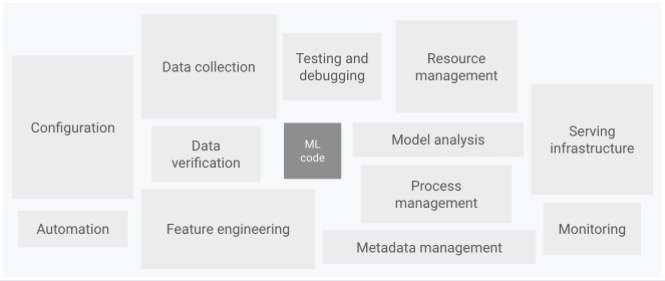
\includegraphics[width=12cm]{images/ml_system.png}    
\end{center}

$\Rightarrow$ \textbf{Continuous Integration (CI):} Automated and frequent integration of code changes into a shared codebase, typically multiple times a day:
\begin{itemize}
    \item Automated unit and integration testing
    \item Early detection of bugs or conflicts
    \item Version control integration (e.g., Git)
    \item Ensures that code remains deployable at all times
    \item \textit{In ML systems CI expands to:}
    \begin{itemize}
        \item Testing of data pipelines
        \item Validation of feature transformations
        \item Evaluation of trained models (performance metrics, fairness, etc)
        \item Reproducibility of training runs
    \end{itemize}
\end{itemize}

$\Rightarrow$ \textbf{Continuous delivery (CD):} Automated releases of tesed software to production-like environments with minimal manual intervention:
\begin{itemize}
    \item CI pipeline results in ana artifact (e.g., Docker image or executable) ready for deployment
    \item CD ensures the artifact can be deployed on-demand
    \item \textit{In ML:}
    \begin{itemize}
        \item Cd involves deployment of entire ML pipelines, \textit{not just code}
        \item Final deployed artifact includes trained model, its metadata, and potentially preprocessing logic
        \item Guarantee model compatibility with input data schemas and operational infrastructure
    \end{itemize}
\end{itemize}


\textit{Why do ML systems decay?} Often refere to as model drift, data drift, concept drift:
\begin{itemize}
    \item \textbf{Data Drift:} Distribution input features changes over time (e.g., user behavior shifts)
    \item \textbf{Label Drift:} Distribution of output labels changes (e.g., fraud patterns evolve)
    \item \textbf{Concept Drift:} Relationship between inputs and outputs changes
    \item \textbf{Upstream Changes:}  Feature pipelines, sensors, third-party APIs change format or quality
    \item \textbf{Label leakage or spurious correlations=:} a model trained on historial correlations may no longer genralize
    \item \textbf{Sampling bias:} Training data is no longer representative of real-world data
\end{itemize}

\subsection*{Modeling Performance Decay Over Time}

Let:
\begin{itemize}
    \item $M_t$ be the model at time $t$
    \item $\mathcal{L}(M_t, \mathcal{D}_t)$ be the loss or error function
    \item $A(t)$ be the accuracy/performance metric (e.g., AUROC)
\end{itemize}

Then, model decay over time can be modeled as:
\[
\frac{dA(t)}{dt} < 0
\]

Or, for exponential decay (simplified):
\[
A(t) = A_0 \cdot e^{-\lambda t}
\]
Where:
\begin{itemize}
    \item $A_0$ is initial performance (e.g., accuracy at deployment)
    \item $\lambda$ is the decay rate, which can be empirically estimated
    \item $t$ is time since deployment
\end{itemize}

Decay rate $\lambda$ can be estimated using performance logs over time via regression or time-series methods.

\subsection*{Retraining Trigger Criteria}

Let:
\begin{itemize}
    \item $A_{\text{current}} =$ current model performance
    \item $A_{\text{threshold}} =$ acceptable performance threshold
\end{itemize}

Then, retraining is triggered when:
\[
A_{\text{current}} < A_{\text{threshold}} \quad \text{or} \quad D_{\text{KL}}\left(P_{\text{train}}(X) \| P_{\text{prod}}(X)\right) > \epsilon
\]

Where $D_{\text{KL}}$ is the Kullback--Leibler divergence between feature distributions.

\section{Information}

\textbf{Shannon's source coding theorem:} Establishes the theoretical limit of data compression for a source of independent, identically-distributed (i.i.d) random variables stating data can be compressed to its Shannon entropy rate with arbitrarily low error probability as the data sequence length approaches infinity 

\textit{"Random variables can be dependent but have $0$ correlation} $\Rightarrow$ Happends when \textbf{dependence is nonlinear and Pearson correlation} (which measures \textit{linear association}) fails to capture it.

\vspace{0.3cm}

\textbf{\textit{Correlation (Pearson): Measures linear dependence between $X$ and $Y$}}

\[
\text{Corr}(X, Y) = \frac{\text{Cov}(X, Y)}{\sigma_X \sigma_Y}
= \frac{\mathbb{E}[(X - \mu_X)(Y - \mu_Y)]}{\sigma_X \sigma_Y}
\]

$\text{Corr}(X,Y) = 0 \Rightarrow$ No \textbf{linear} relationship, NOT necessarily no relationship at all

\vspace{0.2cm}

Two random variables X and Y can satisfy:
\[
\text{Corr}(X, Y) = 0 \quad \text{but} \quad X \not\!\perp\!\!\!\perp Y 
\]
($0$ correlation does NOT imply independence)

It implies complete lack of \textit{statistical dependence} - nonlinear, functional, hidden, monotonic, etc.

\vspace{0.3cm}

$\bullet$ If X and Y are \textbf{independent} then:
\[
\mathbb{E}[XY] = \mathbb{E}[X] \cdot \mathbb{E}[Y] \Rightarrow \text{Cov}(X,Y) = 0
\Rightarrow \text{Corr}(X,Y) = 0
\]
Expected value of their product factorizes

But $\text{Corr}(X,Y) = 0 \not\Rightarrow X \perp\!\!\!\perp Y$ only tells: \textbf{linear component} of relationship is \textit{absent} but $Y$ could still depend on $X$ \textbf{nonlinearly}

\textit{Pearson fails to detect:}
\begin{itemize}
    \item Quadratic
    \item Periodic 
    \item Piecewise
    \item Absolute-value shaped dependencies
    \item Mixture dependencies
\end{itemize}

\exm{Correlation and Independence}{
\begin{center}
$X \sim \mathcal{N}(0,1), \quad Y = X^2$ 

$X \sim N(0,1)$

$Y = X^2$
\end{center}
Then:
\begin{center}
    $\mathbb{E}[X] = 0, \mathbb{E}[Y] = \mathbb{E}[X^2] = 1$
    
    $\text{Cov}(X, Y) = \mathbb{E}[XY] - \mathbb{E}[X]\mathbb{E}[Y] = \mathbb{E}[X^3] = 0$
\end{center}
Thus:
\begin{center}
    $Corr(X,Y)=0$
\end{center}
\begin{center}
    $Y$ is completely determined by $X$ $\cap$ \textbf{not independent}

    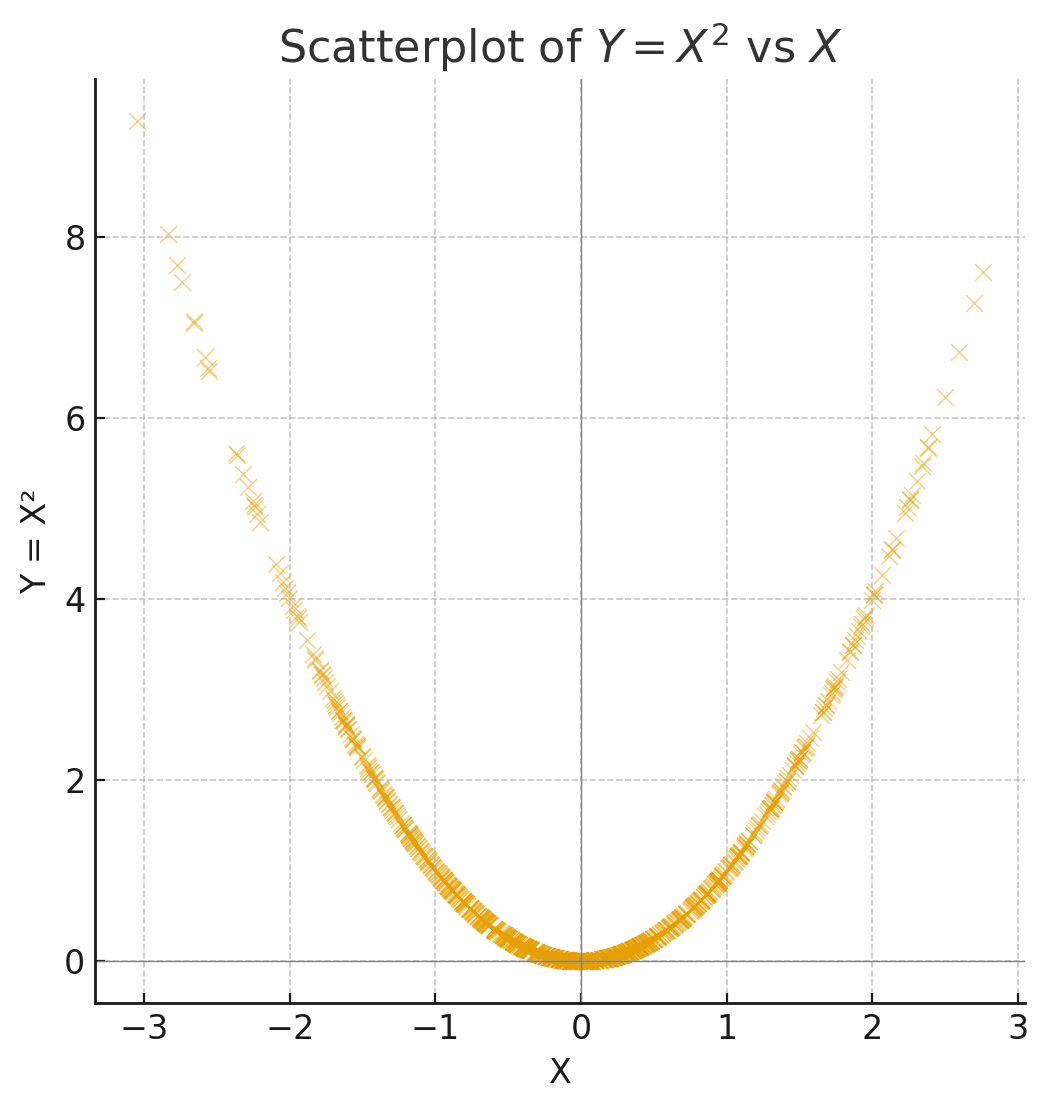
\includegraphics[width=5cm]{images/graphical_demo.png}

    \begin{itemize}
        \item Nonlinear relationship (symmetric parabola)
        \item Pearson $=0$ - positive slope on right $(X>0)$ is canceled by negative on left $(X<0)$
        \item thus, linear trend $=0$ but statistical dependence is \textbf{strong}
    \end{itemize}
\end{center}
}

\textbf{Level 0 MLOps:}
\begin{center}
    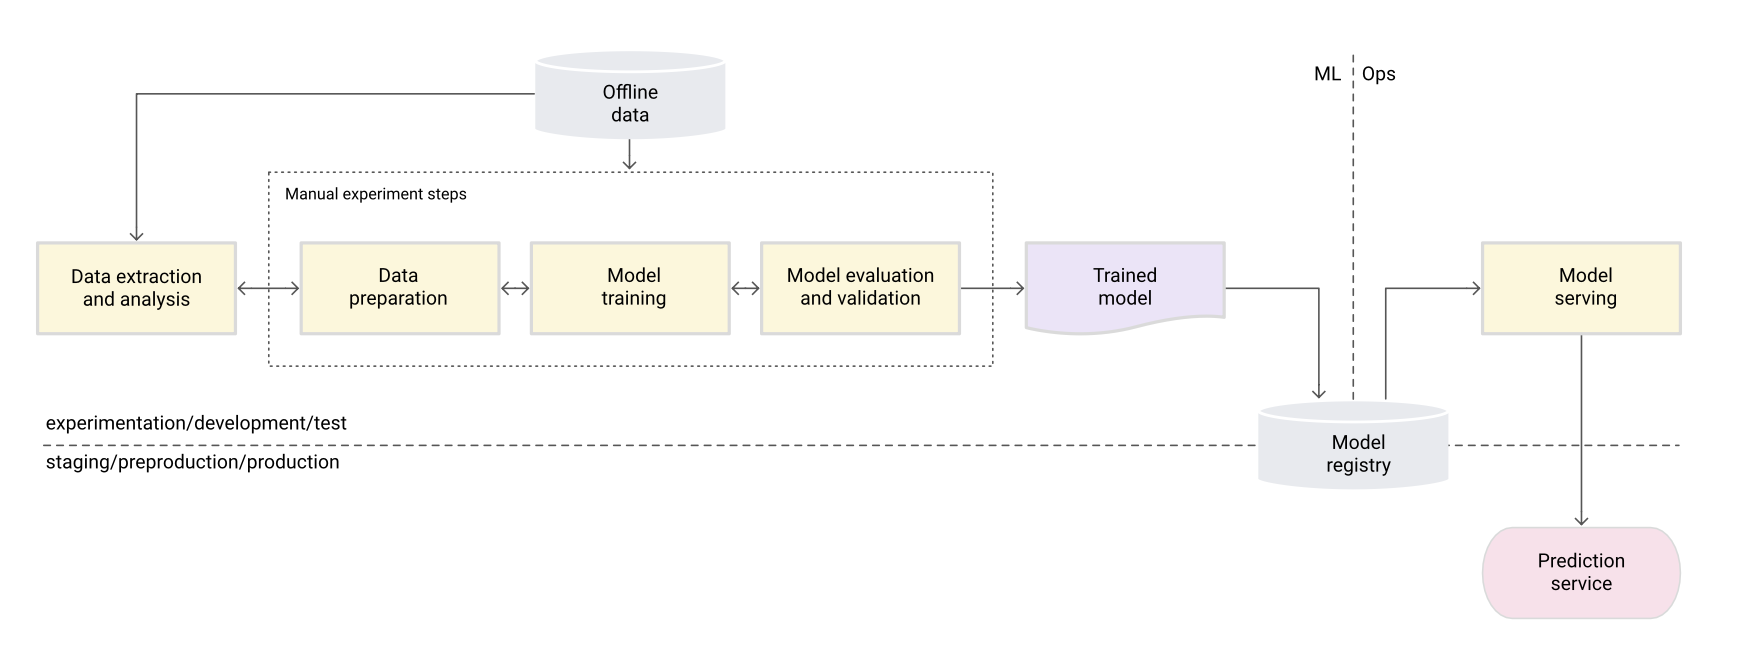
\includegraphics[width=15cm]{images/LEVEL_0.png}
\end{center}

\textbf{Training-Serving Skew:} Difference between performance during training and performance during serving. May be caused by:

\begin{itemize}
    \item Discrepancy between how one handles the data in the training and serving pipelines
    \item change in data between when it was trained and when it was served
    \item feedback loop between model and algorithm
    \item \textbf{Save set of features used at serving and then pipeline such features to a log to use them at training time in order to address issue}
\end{itemize}

\textbf{Level 1 MLOps:}
\begin{center}
    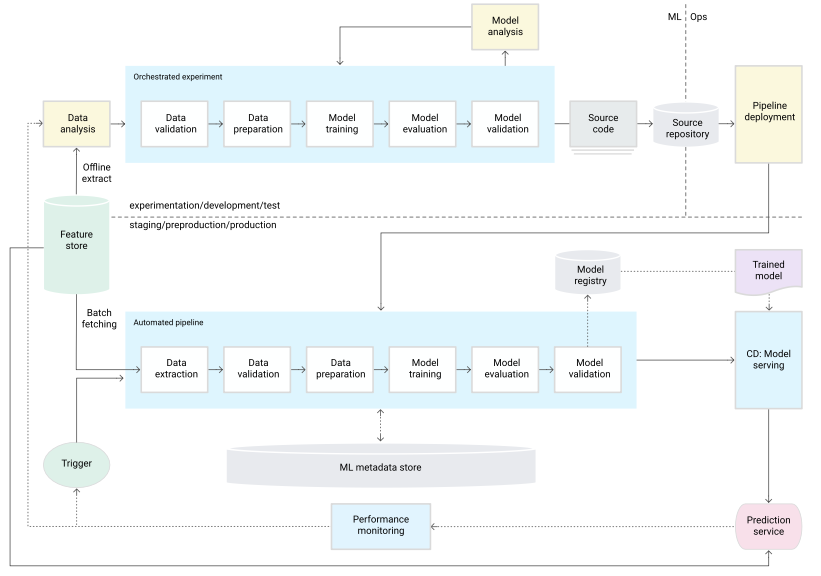
\includegraphics[width=15cm]{images/level_1.png}
\end{center}

Goal is perform continuous training of the model by automating the ML pipeline.

\begin{itemize}
    \item \textbf{CI (Continuous integration):} Every code change is automatically built, tested, validated $\Rightarrow$ Ensures integration errors are caught early
    \item \textbf{CD (Continuous Delivery (or Deployment):} Automates release of validated changes into staging or production
    \item \textbf{CT (Continuous Training):} Extension of \textit{CI/CD} for ML
    \begin{itemize}
        \item automates retraining of models when new data arrives, when performance degrades, or when code/features change
        \item keeps model updated without manual intervention
    \end{itemize}
    \end{itemize}

$\Rightarrow$ \textbf{\textit{Pipeline implementation that is used in the development or experiment environment is used in the preproduction and production environment}}

\vspace{0.3cm}

\textbf{Feature Store:} Centralized repository where you standardize the definition, storage, access for training and serving. It needs to provide API for high-throughput batch serving and low-latency real-time serving for the feature values \& to support both training and serving workloads

\vspace{0.2cm}

\textbf{Metadata Management:} Recorded info about each execution of the ML pipeline in order to help with data and artifacts lineage, reproducibility, and comparisons 

\vspace{0.2cm}

\textbf{Level 2 MLOps:} Implementation of pipeline using CI/CD which has the charachteristics of the automated ML pipelines $+$ the automated CI/CD routines 
\begin{center}
    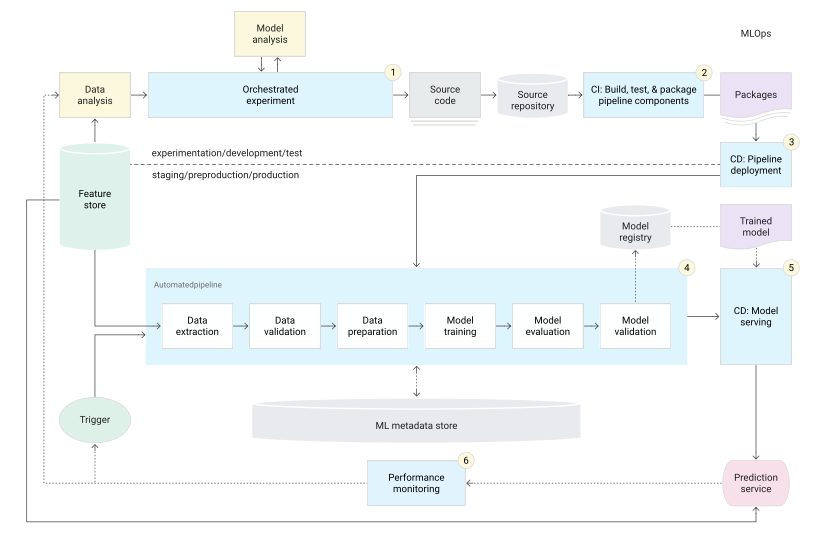
\includegraphics[width=15cm]{images/level_2.png}
\end{center}

\begin{center}
    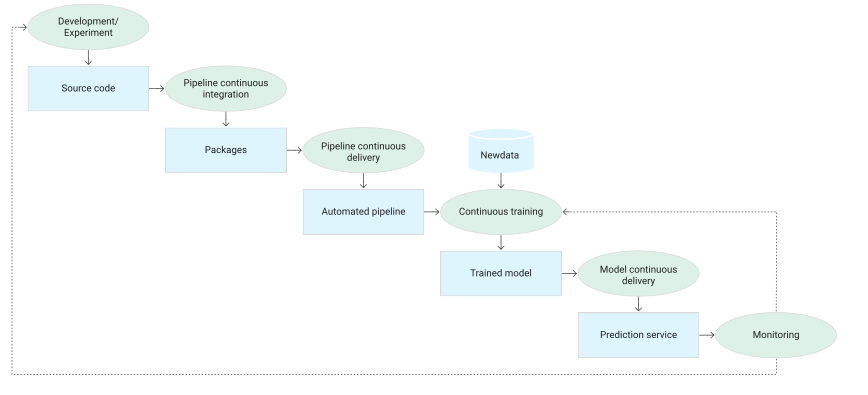
\includegraphics[width=15cm]{images/summary_automation.png}
\end{center}
\end{document}